\section{Methods and Results}
\subsection{Spectroscopy}
%Check which of the CHARM methods are actually needed here and potentially don't bother with them all
\subsubsection{IR Spectroscopy}
\begin{figure}[htbp]
  \centering
  \includegraphics[width=0.8\textwidth]{Images/IR_Basics.png}
  \caption{From \cite{berthomieu_fourier_2009}}
  \label{fig:my-label}
\end{figure}

\begin{figure}[htbp]
  \centering
  \includegraphics[width=0.8\textwidth]{Images/Cystine_IR_pH_dep.png}
  \caption{From \cite{wolpert_infrared_2006}}
  \label{fig:my-label}
\end{figure}


% \begin{figure}[htbp]
%   \centering
%   \includegraphics[width=0.8\textwidth]{Images/he_17_scale.png}
%   \caption{Caption}
%   \label{fig:my-label}
% \end{figure}

% \begin{figure}[htbp]
%   \centering
%   \includegraphics[width=0.8\textwidth]{Images/Predicton_17.png}
%   \caption{Caption}
%   \label{fig:my-label}
% \end{figure}

% \begin{figure}[htbp] 
%     \centering 
%     \includegraphics[width=0.8\textwidth]{Images/sample_17_False_IR.png} 
%     \caption{Caption} \label{fig:my-label}
% \end{figure}

% \begin{figure}[htbp] 
%     \centering 
%     \includegraphics[width=0.8\textwidth]{Images/sample_20_False_IR.png} 
%     \caption{Caption} \label{fig:my-label} 
% \end{figure}

% \begin{figure}[htbp] 
%     \centering 
%     \includegraphics[width=0.8\textwidth]{Images/sample_35_False_IR.png} 
%     \caption{Caption} \label{fig:my-label} 
% \end{figure}

\begin{figure}[htbp] 
    \centering 
    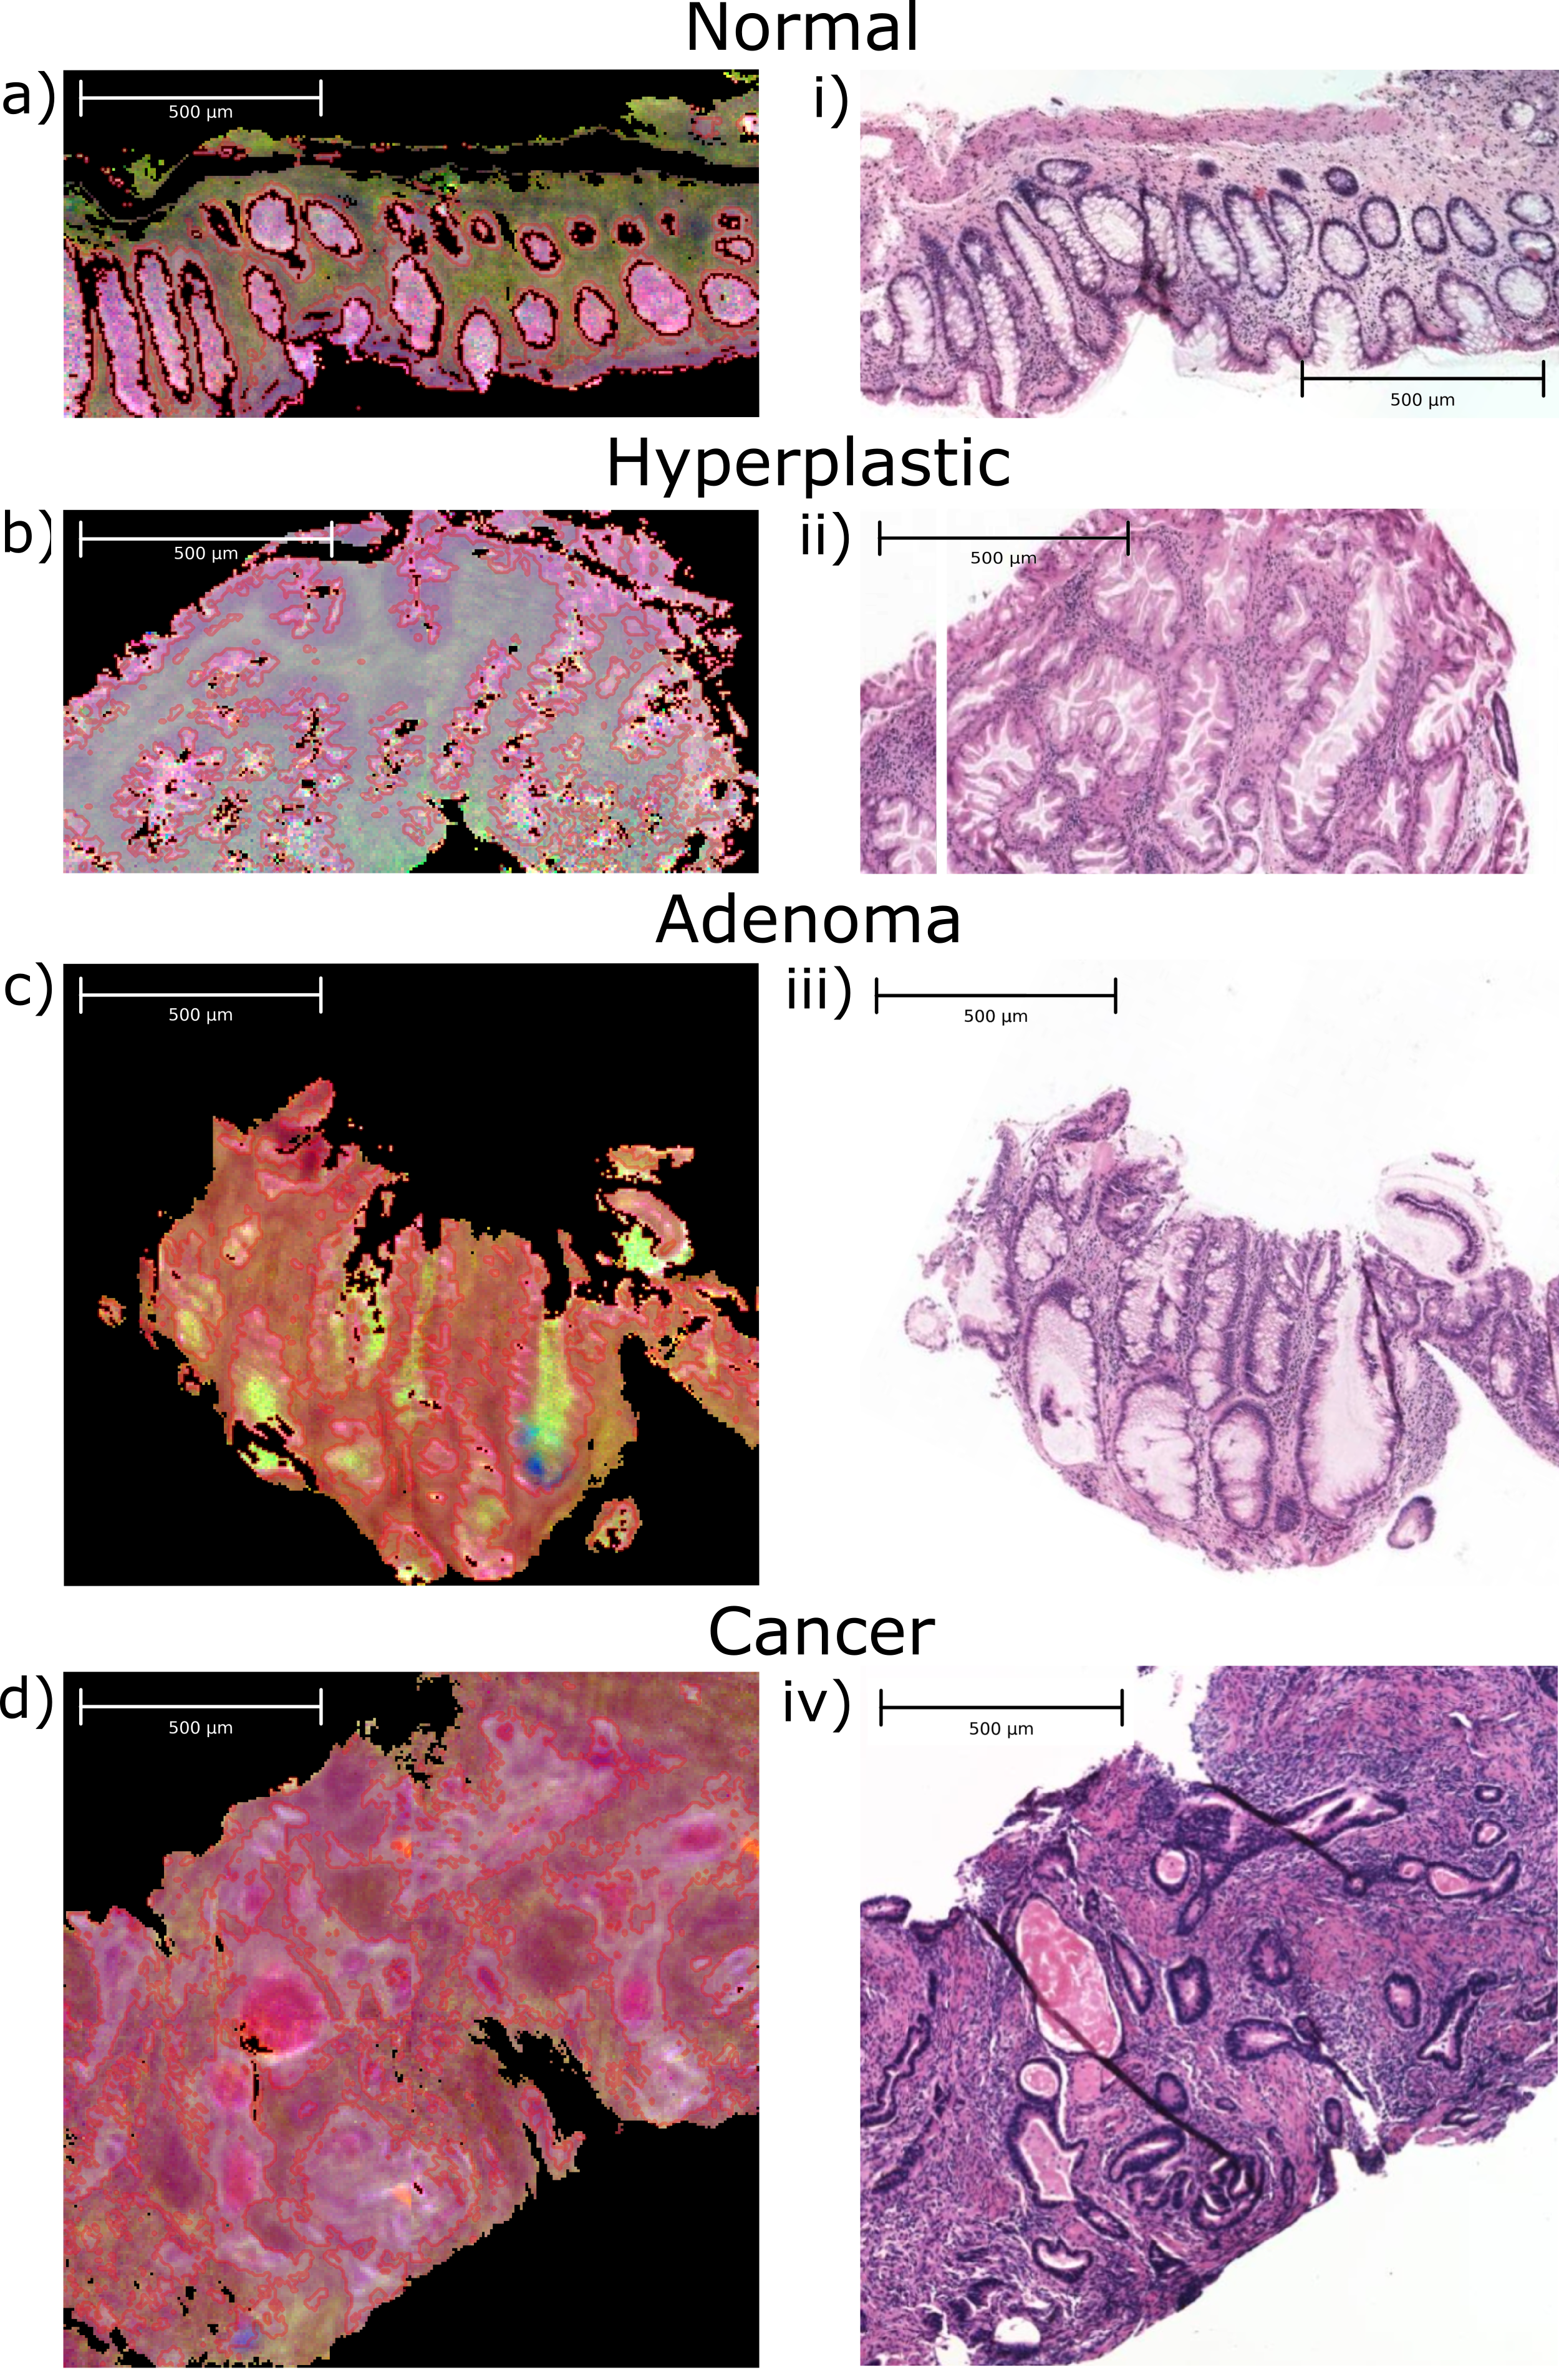
\includegraphics[width=0.9\textwidth]{Images/IR_and_HE_categories.png} 
    \caption{Caption} \label{fig:my-label} 
\end{figure}

\subsubsection{Raman Spectroscopy}
\subsubsection{TPEF}
\subsubsection{SHG}

\subsection{Classical ML Methods for Spectral Classification}

\begin{table}[ht] \centering \caption{Sensitivity and specificity (mean ± SD)
for each model.} \label{tab:model_performance} \begin{tabular}{@{}l l c c c c
c@{}} \toprule Model & Metric & Normal & Adenoma & Hyperplastic & Cancer &
Accuracy \\ \midrule \multirow{2}{*}{PCA~$>$~LDA} & Sensitivity & 42 (20.4) & 84
(14.3) & 31 (17.7) & 39 (26.3) & 61 (7.6) \\ & Specificity & 90 (11.1) & 57 (19.
9) & 94 (5.4) & 95 (6.2) & — \\ \midrule \multirow{2}{*}{XGBoost} & Sensitivity
& 58 (11.9) & 80 (14.4) & 41 (14.7) & 62 (33.6) & 68 (10.0) \\ & Specificity &
88 (6.6) & 77 (10.2) & 91 (2.6) & 96 (6.2) & — \\ \midrule \multirow{2}{*}{PCA~$>$~XGBoost} & Sensitivity & 43 (11.5) & 55 (11.9) & 28 (11.9) & 75 (20.9) & 51 (9.
2) \\ & Specificity & 88 (10.3) & 79 (7.7) & 90 (6.7) & 77 (10.5) & — \\
\bottomrule \end{tabular} \end{table}


% Include the other methods here
\subsubsection{XGBoost}
\subsubsection{Spectral Matching}


\subsection{Deep Learning Methods for Spectral Classification}
\subsubsection{Dataset Challenges}
\begin{figure}[htbp]
  \centering
  \includegraphics[width=0.8\textwidth]{Images/Dataset_Class_Differences.png}
  \caption{Caption}
  \label{fig:my-label}
\end{figure}

\subsubsection{De-noising Methods}
\subsubsection{Evaluation Metrics}

\subsubsection{Model Architecture}
\begin{figure}[htbp]
  \centering
  \includegraphics[width=0.8\textwidth]{Images/SCNN_TPL_Arch.png}
  \caption{Caption}
  \label{fig:my-label}
\end{figure}

\begin{figure}[htbp]
  \centering
  \includegraphics[width=0.8\textwidth]{Images/Tanh_Relu_Demo.png}
  \caption{Caption}
  \label{fig:my-label}
\end{figure}
\subsubsection{Regularisation Techniques}

\begin{figure}[htbp] 
    \centering 
    \includegraphics[width=0.8\textwidth]{Images/best_val_accuracy.png} 
    \caption{Caption} \label{fig:my-label}
\end{figure}

\begin{table}[ht] \centering \caption{Metrics for single fold test set
with 50\% voting threshold and no label smoothing} \begin{tabular}{lcccc} \toprule Metric & Normal &
Adenoma & Hyperplastic & Cancer \\ \midrule Accuracy & 0.699 & 0.699 & 0.680 & 0.945
\\ Sensitivity & 0.662 & 0.452 & 0.258 & 0.783 \\ Specificity & 0.708 & 0.936 &
0.762 & 0.972 \\ False positive rate & 0.292 & 0.064 & 0.238 & 0.028 \\ \midrule
Overall Accuracy & \multicolumn{4}{c}{0.5387} \\ \bottomrule \end{tabular}
\label{tab:voting05_results} \end{table}

\begin{table}[ht] \centering \caption{Metrics for single fold test set with 50\% voting threshold and 10\% label smoothing} \begin{tabular}{lcccc} \toprule Metric & Normal
& Adenoma & Hyperplastic & Cancer \\ \midrule Accuracy & 0.702 & 0.700 & 0.674 & 0.
944 \\ Sensitivity & 0.643 & 0.458 & 0.257 & 0.782 \\ Specificity & 0.716 & 0.
933 & 0.755 & 0.971 \\ False positive rate & 0.284 & 0.067 & 0.245 & 0.029 \\
\midrule Overall Accuracy & \multicolumn{4}{c}{0.5349} \\ \bottomrule
\end{tabular} \label{tab:ls01_results} \end{table}

\begin{table}[ht] \centering \caption{Metrics for single fold test set with 50\% voting threshold and 20\% label smoothing} \begin{tabular}{lcccc} \toprule Metric & Normal
& Adenoma & Hyperplastic & Cancer \\ \midrule Accuracy & 0.700 & 0.692 & 0.672 & 0.
941 \\ Sensitivity & 0.650 & 0.436 & 0.266 & 0.786 \\ Specificity & 0.713 & 0.
937 & 0.751 & 0.967 \\ False positive rate & 0.287 & 0.063 & 0.249 & 0.033 \\
\midrule Overall Accuracy & \multicolumn{4}{c}{0.5345} \\ \bottomrule
\end{tabular} \label{tab:ls02_results} \end{table}


\subsubsection{Model Performance}

\begin{figure}[htbp] 
    \centering 
    \includegraphics[width=0.8\textwidth]{Images/Categorisation_train_test.png} 
    \caption{Caption} \label{fig:my-label} 
\end{figure}

\begin{figure}[htbp] 
    \centering 
    \includegraphics[width=0.8\textwidth]{Images/Confidence.png} 
    \caption{Caption} \label{fig:my-label}
\end{figure}

\begin{table}[ht] \centering \caption{XGBoost} \label{tab:xgboost}
\begin{tabular}{lcccc} \toprule & \textbf{Normal} & \textbf{Adenoma} &
\textbf{Hyperplastic} & \textbf{Cancer} \\ \midrule \textbf{Acc} & $0.809\pm0.
026$ & $0.749\pm0.073$ & $0.826\pm0.011$ & $0.888\pm0.055$ \\ \textbf{Sens} & $0.
490\pm0.115$ & $0.781\pm0.055$ & $0.386\pm0.133$ & $0.603\pm0.091$ \\
\textbf{Spec} & $0.886\pm0.029$ & $0.711\pm0.104$ & $0.911\pm0.036$ & $0.937\pm0.
057$ \\ \textbf{FPR} & $0.115\pm0.029$ & $0.289\pm0.104$ & $0.090\pm0.036$ & $0.
063\pm0.057$ \\ \midrule \multicolumn{5}{c}{\textbf{Overall Weighted Accuracy:}
$0.565\pm0.058$} \\ \bottomrule \end{tabular} \end{table}

\begin{table}[ht] \centering \caption{SCNN} \label{tab:scnn_tpl3}
\begin{tabular}{lcccc} \toprule & \textbf{Normal} & \textbf{Adenoma} &
\textbf{Hyperplastic} & \textbf{Cancer} \\ \midrule \textbf{Acc} & $0.756\pm0.
071$ & $0.707\pm0.017$ & $0.801\pm0.083$ & $0.881\pm0.070$ \\ \textbf{Sens} & $0.
739\pm0.111$ & $0.527\pm0.071$ & $0.323\pm0.069$ & $0.777\pm0.082$ \\
\textbf{Spec} & $0.760\pm0.101$ & $0.883\pm0.089$ & $0.894\pm0.095$ & $0.899\pm0.
072$ \\ \textbf{FPR} & $0.240\pm0.102$ & $0.118\pm0.089$ & $0.107\pm0.095$ & $0.
102\pm0.072$ \\ \midrule \multicolumn{5}{c}{\textbf{Overall Weighted Accuracy:}
$0.591\pm0.003$} \\ \bottomrule \end{tabular} \end{table}


\subsection{Explainability}
% A bit of background on why explainability is important and why it must be used in medical contexts
\subsubsection{Local Interpretable Model-Agnostic Explanations}
\begin{figure}[htbp]
  \centering
  \includegraphics[width=0.8\textwidth]{Images/lime_explanation.png}
  \caption{From \cite{ribeiro_why_2016}}
  \label{fig:my-label}
\end{figure}

\begin{figure}[htbp]
  \centering
  \includegraphics[width=0.8\textwidth]{Images/lime_demo.png}
  \caption{Caption}
  \label{fig:my-label}
\end{figure}

\subsubsection{CRIME}
\begin{figure}[htbp]
  \centering
  \includegraphics[width=1\textwidth]{Images/crime_umap.png}
  \caption{Caption}
  \label{fig:my-label}
\end{figure}
\subsubsection{VAE Methods}
\paragraph{Clustering VAE Approaches}

\begin{figure}[htbp]
  \centering
  \includegraphics[width=1\textwidth]{Images/crime_groupings_by_category_100.png}
  \caption{Caption}
  \label{fig:my-label}
\end{figure}

\begin{figure}[htbp] 
    \centering 
    \includegraphics[width=1\textwidth]{Images/crime_lime_plots.png} 
    \caption{Caption}
\label{fig:my-label} \end{figure}

\begin{figure}[htbp]
    \centering
    \includegraphics[width=1\textwidth]{Images/context_model_metrics.png}
    \caption{Caption} \label{fig:my-label} 
\end{figure}

\paragraph{Logic Explained Networks}